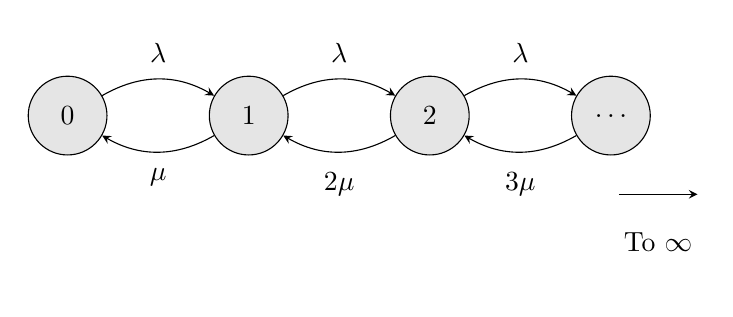
\begin{tikzpicture}[>=stealth, node distance=2.3cm, every node/.style={circle}]
    % Nodes
    \node (0) [{draw, fill=gray!20, minimum size=10mm, inner sep=0pt}] {0};
    \node (1) [{right of=0, draw, fill=gray!20, minimum size=10mm, inner sep=0pt}] {1};
    \node (2) [{right of=1, draw, fill=gray!20, minimum size=10mm, inner sep=0pt}] {2};
    \node (3) [{right of=2, draw, fill=gray!20, minimum size=10mm, inner sep=0pt}] {$\dots$};
    
    % Transition arrows for arrivals
    \draw[->] (0) to[bend left] node[above] {$\lambda$} (1);
    \draw[->] (1) to[bend left] node[above] {$\lambda$} (2);
    \draw[->] (2) to[bend left] node[above] {$\lambda$} (3);
    \draw[->] (7, -1) -- (8, -1) node[below, midway] {To $\infty$};
    

    % Transition arrows for departures
    \draw[->] (1) to[bend left] node[below] {$\mu$} (0);
    \draw[->] (2) to[bend left] node[below] {$2\mu$} (1);
    \draw[->] (3) to[bend left] node[below] {$3\mu$} (2);
    
\end{tikzpicture}
